\documentclass{article}
\usepackage[utf8]{inputenc}
\usepackage[spanish]{babel}
\usepackage{natbib}
\usepackage{graphicx}
\usepackage{mathtools}
\usepackage{color}
\usepackage{float}
\usepackage{fancyhdr}
\usepackage{adjustbox}
\usepackage{dsfont}
\usepackage{verbatim}

\pagestyle{fancy}
\lhead{Grupo 4 - Turno 7}
\chead{Trabajo Practico Nro 6}
\rhead{Primer Cuatrimestre 2015}

\begin{document}

\section{Introducción Teórica}
La corrientes dependientes del tiempo son todas aquellas cuyos valores no son constantes respecto al mismo. En la realidad, este tipo de corrientes son las más comunes y aquellas que nos proporcionan tanto electricidad en los hogares, como diversos servicios tales como radio, televisión, entre otros.
Dado que las corrientes suelen ser de forma sinusoidal (y las diferencias de tensión que las generan), se recurre a los números complejos para facilitar los cálculos de las mismas. De esta manera, se define el término de \textit{impedancia} cuyo valor depende del elemento circuital al que corresponda, siendo al misma:

\begin{equation}
\mathds{Z}_R = R
\end{equation}

\begin{equation}
\mathds{Z}_C = \frac{-j}{\omega C}
\end{equation}

\begin{equation}
\mathds{Z}_L = j \omega L
\end{equation}



Y siendo el valor total de la impedancia del circuito:

\begin{equation}
\mathds{Z} = \mathds{Z}_R + \mathds{Z}_C + \mathds{Z}_L
\end{equation}

De esta manera, un circuito será resistivo si su impedancia es real, capacitivo si su parte imaginaria es negativa e inductivo si su parte imaginaria es positiva. 
\\
Y siendo:

\begin{equation}
\mathds{I} = io  e^{j\varphi_i}
\end{equation}

Por último, esto lleva a una "reestructuración" de la ley de Ohm a la \textit{ley de Ohm compleja}:

\begin{equation}
\mathds{E} = \mathds{IZ}
\end{equation}


\section{Objetivos}
Los objetivos de la experiencia refieren a observar aquellos fenómenos de corrientes que varían en el tiempo (sean transitorias o alternas) vistos de forma teórica en la materia, en particular:
    \begin{itemize}
		\item El funcionamiento de un circuito RLC.
		\item El uso de los transformadores y su forma de implementación.
		\item Los valores que se obtienen al asociar inductancias de acoplamiento.
		\item El proceso de carga y descarga de un capacitor.
	\end{itemize}

\section{Materiales}
	Para la experiencia se utilizaron los siguientes materiales:
    \begin{itemize}
		\item Inductancias de 400 espiras.
		\item Núcleos de materiales mangnéticos (en forma de O y de E).
		\item Capacitor.
		\item Resistencia.
		\item Osciloscopio.
		\item Generador de funciones.
	\end{itemize}

\section{Desarrollo}

\subsection{Respuesta en frecuencia de un circuito RLC serie}

En esta parte del trabajo, se midieron los elementos y se armó un circuito RLC serie. Llevamos al circuito a resonancia y comenzamos a variar la frecuencia que proveyó el generador de funciones con el objetivo de variar el voltaje $V_r$ subiendo y bajando f. 

Cabe aclarar que obtuvimos el valor para la frecuencia de resonancia teórica por medio de la ecuación:
\begin{equation}
f_0teo = \frac{1}{2 \pi \sqrt{LC}} = 19232,61 hz
\end{equation}

Una vez terminadas las mediciones de $\omega$, calculamos f y la caída de tensión $V_r$ teórica para cada caso utilizando:
\begin{equation}
\mathds{E} = \mathds{IZ}
\end{equation}

\begin{equation}
\left |{I}\right |=\frac{V_g}{\sqrt[]{(R+R_g+R_L)^2+(\omega L -\frac{1}{\omega C } )^2}}
\end{equation}


Las mediciones y resultados obtenidos se reflejan en las siguientes tablas:
\begin{table}[H]
\centering
%%%%%%%%%%%%%%%%%%%%%%%%%%%%%%%%%%%%%%%%%%%%%%%%%%%%%%%%%%%%%%%%%%%%%%
%%                                                                  %%
%%  This is a LaTeX2e table fragment exported from Gnumeric.        %%
%%                                                                  %%
%%%%%%%%%%%%%%%%%%%%%%%%%%%%%%%%%%%%%%%%%%%%%%%%%%%%%%%%%%%%%%%%%%%%%%
\begin{tabular}{|c|c|c|c|}
\hline
Variación	&Frecuencia por encima $f_0$ (hz)	&$V_r$ teórico	&$V_r$ experimental\\ \hline
100,00\%	&20000	&1,89	&2\\
90,00\%	&16043  	&1,88	&1,8\\
80,00\%	&13250	    &1,83	&1,60\\
70,00\%	&10080	    &1,69	&1,40\\
60,00\%	&8192	&1,56	&1,20\\
50,00\%	&7500	&1,49	&1,00\\
40,00\%	&6134	&1,33	&0,80\\ \hline
\end{tabular}


\caption{Resultados para caídas de tensión teóricas por encima de $f_0$}
\end{table}

\begin{table}[H]
\centering
%%%%%%%%%%%%%%%%%%%%%%%%%%%%%%%%%%%%%%%%%%%%%%%%%%%%%%%%%%%%%%%%%%%%%%
%%                                                                  %%
%%  This is a LaTeX2e table fragment exported from Gnumeric.        %%
%%                                                                  %%
%%%%%%%%%%%%%%%%%%%%%%%%%%%%%%%%%%%%%%%%%%%%%%%%%%%%%%%%%%%%%%%%%%%%%%
\begin{tabular}{|c|c|c|c|}
\hline
Variación	&Frecuencia por debajo $f_0$ (hz)	&$V_r$ teórico	&$V_r$ experimental	\\ \hline
100,00\%	&20000	&1,89	&2,00	\\
90,00\%	&24416	&1,87	&1,80	\\
80,00\%	&26920	&1,84	&1,60	\\
70,00\%	&34201	&1,73	&1,40	\\
60,00\%	&41230	&1,62	&1,20	\\
50,00\%	&54703	&1,41	&1,00	\\
40,00\%	&62249	&1,31	&0,80	\\\hline
\end{tabular}


\caption{Resultados para caídas de tensión teóricas por debajo de $f_0$}
\end{table}

A continuación graficamos los valores para $V_r$ en función de f. Los resultados \textcolor{red}{experimentales se representan en rojo} y los \textcolor{blue}{teóricos se representan en azul}.
\begin{figure}[H]
\centering
\includegraphics[scale=0.8]{curva}
\caption{Variación de la frecuencia experimental}
\end{figure}
Si bien en teoría, los valores de subida y de bajada con respecto a $f_{0}$ deberían ser simétricos, en la practica esto no ocurre y por eso se llega a esta curva.

Con los datos experimentales obtenidos, pudimos además obtener un valor para el factor de mérito Q experimental y teórico calculándolos como:
\begin{equation}
Q_{exp} = \frac{f_0}{f_2 - f_1} = 0,39
\end{equation}
Donde $f_{2}$ y $f_{1}$ son las frecuencias de media potencia obtenidas con $V_{r}$ al 70 $\%$.

\begin{equation}
Q_{teo} = \frac{2 \pi f_0 L}{R + R_G + R_L} = 0,36
\end{equation}

Finalmente calculamos el error relativo porcentual de las magnitudes f y Q:
\begin{equation}
\varepsilon_Q = \frac{Q_teo - Q_exp}{Q_teo} 100\% = 8,6\%
\end{equation}
\begin{equation}
\varepsilon_f = \frac{f_teo - f_exp}{f_teo} 100\% = 4\%
\end{equation}

\begin{comment}
se pueden realizar distintos cálculos relacionados con corriente, factor de mérito y frecuencias teóricas.
Por un lado, calculamos el factor de mérito Q teórico. El mismo se encuentra en la hoja de datos. Es posible también, calcular este factor de mérito, con resultados experimentales con la fórmula Q=f0/(f2-f1).
Para calcular las frecuencias teóricas, teniendo las de tipo experimental y usando la fórmula de la corriente, sacamos en cada punto porcentual, el valor de la frecuencia teórica de resonancia.
En la siguiente tabla, se encuentran los datos obtenidos.
CHEQUEAR EXPLICACIÓN Y LO QUE PUSE EN GENERAL!!!!!!
Es posible también, con estos valores, realizar la curva de respuesta en frecuencia teórica y experimental.

\textcolor{blue} {Calculamos también, el error porcentual de f0 y Q que se calcularon en base a R,L y C respecto a los obtenidos de forma experimental.}
\end{comment}

\subsection{Transformador}

Para la realización de esta experiencia se utilizaron, en ambos casos, arrollamientos de 400 espiras y frecuencia de un 1kHz. 
En esta experiencia se monto el circuito de la figura \ref{fig:nucleo_c} utilizando el núcleo en forma de C, el cual es solo
un transformador.

\begin{figure}[H]
\centering
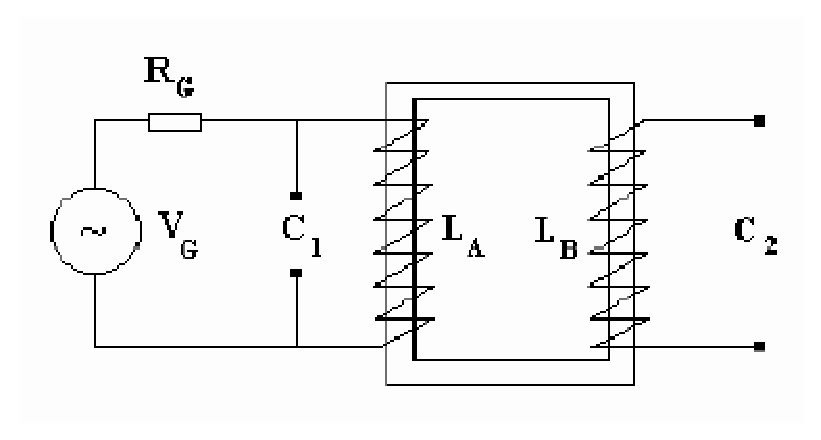
\includegraphics[width=\columnwidth]{transformador_nucleo_c}
\label{fig:nucleo_c}
\end{figure}

Luego se midió la tensión de entrada y la de salida al mismo tiempo para registrar la tensión en bornes del primario y del secundario.

Si bien ambos arrollamientos tienen la misma cantidad de vueltas, existen perdidas y fugas por lo que la siguiente relación no se cumple:
\begin{equation}
\frac{V_{2}}{V_{1}} = \frac{N_{2}}{N_{1}}
\end{equation}

Sino que se tiene:

\begin{equation}
\frac{V_{2}}{V_{1}} = k \frac{N_{2}}{N_{1}}
\end{equation}

Con $k < 1$, conociéndose a k como el \emph{factor de acoplamiento}.

Para este caso se obtuvieron los siguientes resultados:

\begin{align*}
N_{1} = N_{2} = 400 \\
V_{1} =  0.37 V \\ 
V_{2} = 0.22 V \\
k \approx  0.62
\end{align*}

En este caso obtuvimos un factor de acoplamiento de 0.62, aproximadamente. Esto quiere decir que con este tipo de núcleo poseemos un transformador con un rendimiento del 
62\%.

Luego se repitió la experiencia pero colocando ambos arrollamientos en la rama central del núcleo E como muestra la siguiente figura.

\begin{figure}[H]
\centering
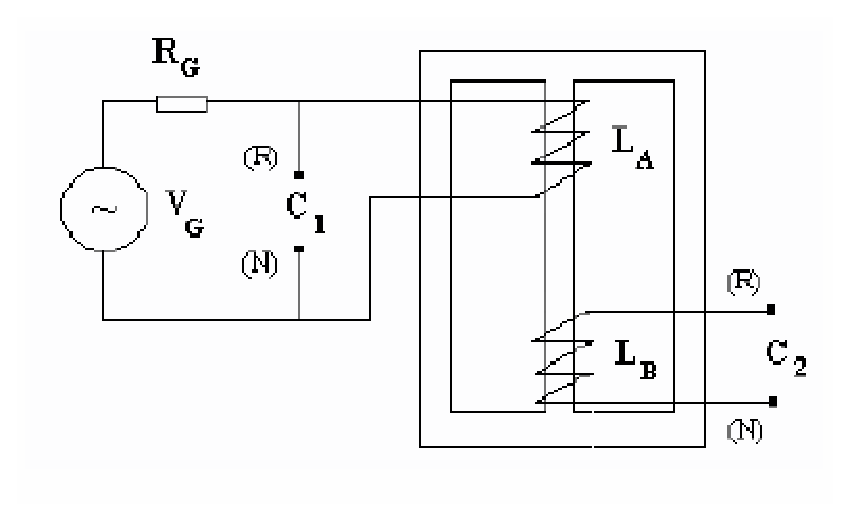
\includegraphics[width=\columnwidth]{transformador_nucleo_e}
\end{figure}

Se obtuvieron los siguientes resultados:

\begin{align*}
N_{1} = N_{2} = 400 \\
V_{1} =  0.42 V \\ 
V_{2} =  0.35 V \\
k \approx  0.83
\end{align*}

Para este ultimo caso, el factor de acoplamiento fue de, aproximadamente, 0.83. Nuevamente, eso quiere decir que con el tipo de núcleo utilizado se posee un transformador con un rendimiento de aproximadamente el 83\%. Esto se debe, mas que nada, por la cercanía de los arrollamientos entre si evitando una fuga o perdida del flujo magnético que los atraviesa. Con este ultimo razonamiento podemos explicar como la configuración del ultimo caso nos permite poseer un transformador con un mayor rendimiento que el del caso anterior, donde se utilizo un núcleo C.

Los V obtenidos, en ambos casos, corresponden a las tensiones eficaces.

\subsection{Asociaciones de inductancias acoplamiento}

Cuando una bobina A concatena parte del flujo magnético generado por una bobina B estamos en presencia del fenómeno de inducción mutua, por el cual variaciones en la corriente en una de las bobinas ($I_A$ ó $I_B$)se refleja en una fem inducida en la otra computable a través de las relaciones:
\begin{equation}
V_A = M \frac{dI_B}{dt} 
\end{equation}
\begin{equation}
V_B = M \frac{dI_A}{dt} 
\end{equation}
Se define al factor de acoplamiento k como la fracción del flujo generador por A que es concatenada por B (la definición inversa brinca el mismo resultado), por lo que el coeficiente de inducción mutua se puede calcular como:
\begin{equation}
M = \sqrt{L_A L_B}
\end{equation}
En esta experiencia, determinamos el factor de acoplamiento midiendo la inductancia total de dos arrollamientos conectados en serie con un núcleo O y uno E.
Comenzamos registrando con el multímetro los valores de $L_A$ y $L_B$, por separado, en el núcleo. Luego medimos el valor de la inductancia total estando conectadas en las dos combinaciones posibles (bornes homólogos y no homólogos). Al medir registramos un valor muy grande y uno más pequeño, deducimos que el grande corresponde al caso en el que los flujos son aditivos, y el pequeño al caso en el que los flujos se contrarrestan. Nombramos a estas mediciones $L_a$ y $L_s$ respectivamente.
Con estos datos, calculamos M como:
\begin{equation}
M = \frac{L_a L_s}{4} 
\end{equation}
y, finalmente, k como:
\begin{equation}
k = \frac{M}{\sqrt{L_A L_B}}
\end{equation}
Los resultados se encuentran en la hoja de datos.\\

\textbf{¿Se obtiene el mismo valor de M y k?} No, los valores obtenidos para los núcleos utilizados son diferentes.\\

\textbf{¿Qué cambió si el material del núcleo es el mismo?} Cambió la geometría del núcleo, las constantes M y L dependen de factores geométricos, tales como tamaño, forma, número de vueltas, posiciones relativas de las dos bobinas y la constante del material $\mu$ en el que estén enrolladas.

\subsection{Transitorios, carga y descarga de un capacitor}
Se armó el siguiente circuito, con la excepción de la resistencia R. En vez de agregar una, se utilizo la que posee el generador. Dicha resistencia es de $50 \Omega$

\begin{figure}
\centering
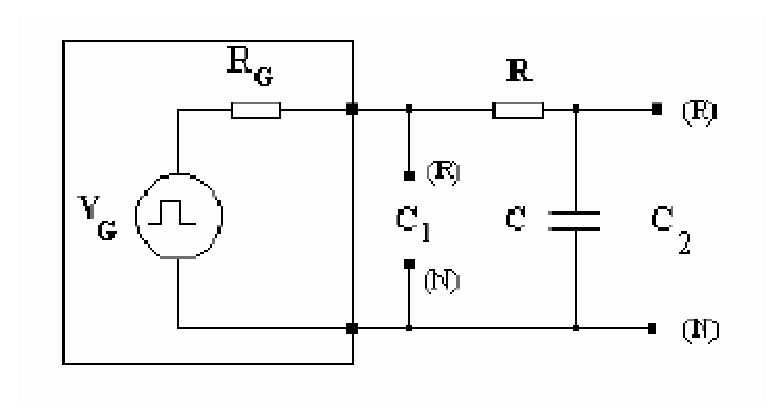
\includegraphics[width=\columnwidth]{experiencia_capacitor}
\caption{Circuito armado, exceptuando por la resistencia R}
\end{figure}

El valor del capacitor, medido con el tester, es de $1,1 nF$. Con los valores de la resistencia y el capacitor calculamos:

\begin{align*}
\tau = RC = 5.5 10^{-5} \\
\frac{1}{RC}  = 18181,8 kHz
\end{align*}

Si en un circuito RC serie el capacitor esta descargado inicialmente entonces la tensión sobre el capacitor vale cero para t = 0 y luego se va cargando como: 

\begin{equation}
V_c = V_g(1-e^{\frac{-t}{RC}})
\end{equation}

Similarmente, si el capacitor se encuentra inicialmente cargado a una tensión inicial Vg y lo descargamos sobre la misma resistencia, la tensión sobre el mismo vale: 

\begin{equation}
V_c = V_g e^{\frac{-t}{RC}}
\end{equation}

Cuando la constante RC es del orden de varios segundos es posible seguir el proceso de carga y descarga del capacitor con un voltímetro conectado a través de los bornes del capacitor, en cambio, si es del orden de pocos segundos sería imposible observarlo y por eso se recurre a un osciloscopio. 

\begin{itemize}
\item ¿Cómo se compara el tiempo de carga o descarga con el valor RC? Si RC es un número grande entonces $\frac{-t}{RC}$ será muy pequeño y la tensión sobre el capacitor se aproximará a cero. A medida que aumenta t, la tensión sobre C se acercará a la tensión entregada por el generador hasta que esté totalmente cargado. Si RC es muy pequeña, la tensión sobre el capacitor y la del generador se parecen mucho mas a medida que aumenta el t. 
\item Aplicamos una frecuencia de excitación $f < \frac{1}{RC}$ 
\end{itemize}

\textbf{¿Qué relación debe haber entre f y RC para que la tensión máxima sobre el capacitor sea superior al 90\% de la entregada por el generador?}

\begin{align*}
|I| = \frac{V_c}{X_c} = \frac{V_g}{Z_t} \\
|V_c| = \frac{\frac{|V_g|}{wC}}{\sqrt{R^2+(\frac{1}{wC})^2}} = \frac{|V_g|}{\sqrt{R^2 w^2 C^2 +1}}\\
\frac{1}{\sqrt{R^2 w^2 C^2 +1}} > 0,9 \\
f < \frac{1}{\sqrt{2 \pi RC}} \sqrt{\frac{1}{0,9^2}-1} \\
\end{align*}

\begin{itemize}
\item  Aplicamos una frecuencia $f >> \frac{1}{RC}$.
\end{itemize}
\textbf{ ¿Qué relación matemática aproximada gurda la salida con la entrada?} Al ir aumentando la frecuencia de excitación, la reactancia capacitiva (XC) irá decreciendo, entonces los efectos capacitivos también decrecen hasta que las tensiones sobre la resistencia y sobre la entrada se igualan.

Tomamos el voltaje de salida sobre el canal 2 
\begin{equation}
V_{c2} = I_{max} X_c = \frac{I_{max}}{wC}
\end{equation}

el voltaje de entrada es dado por el generador por medio del canal 1: 

\begin{equation}
V_{c1} = I_{max} Z_t = I_{max}\sqrt{R^2 + \frac{1}{wC}}
\end{equation}

La relación entre la tensión de entrada y salida es:

\begin{equation}
\frac{V_{C2}}{V_{C1}} = \frac{\frac{1}{wC}}{\sqrt{R^{2}} + (\frac{1}{wC})^{2}}
\end{equation}

\textbf{¿Cómo se denomina este circuito? ¿Por qué?} 
A este circuito se lo reconoce como filtro paso bajos RC porque al ser la frecuencia muy baja (tendiente a cero) la tensión sobre el capacitor será máxima. Si la frecuencia hubiese sido máxima (tendiente a 
infinito) la tensión sobre el capacitor tenderá a cero. El filtro deja pasar solo frecuencias debajo de 
la frecuencia de corte $\frac{1}{2 \pi RC}$ y elimina las superiores a esta. (Un filtro pasa altos RC en cambio elimina las frecuencias inferiores a la de corte y deja pasar a las superiores) 

\section{Resultados}
Los resultados de la experiencia se encuentran en la hoja de datos adjunta.

\section{Conclusiones}

\begin{itemize}
		\item La forma en que obtenemos los datos, así como el accionar de los operadores del osciloscopio, pueden llevar a errores en las mediciones.
		\item Si bien en teoría los valores de la experiencia uno, deberían ser simétricos (dar lo mismo para las dos mediciones de cada porcentaje), en la realidad esto no es correcto. No se obtienen valores iguales para los porcentajes en ambos sentidos.
		\item Al calcular el error porcentual de f y Q, esperábamos que este fuera mayor. Además, a pesar de ser magnitudes distintas, el error que se comete en el cálculo de Q es el doble al error porcentual de la frecuencia.
		\item En la experiencia del transformador (2), observamos la gran influencia de la disposición de los materiales de un sistema en el rendimiento del mismo. Mientras que cuando los arrollamientos están en dos ejes del núcleo, el factor de acoplamiento es aproximadamente 0,62, cuando los ponemos en un mismo eje el factor aumenta en 0,21. Esto nos hace concluir que si se evita la pérdida de flujo magnético, lo que aumenta el rendimiento.
		\item En la experiencia tres, observamos que los valores de M y K varían, si lo hacen las condiciones de realización del experimento. Entre estas condiciones, se encuentran geometría del núcleo y posición de las bobinas. Al igual que en la experiencia anterior, vemos como la disposición de los materiales influye en los resultados medidos/obtenidos.
		\item El tiempo característico de la experiencia cuatro, es un tiempo inimaginable a nivel "humano". Es mucho menor a un segundo.
\end{itemize}
\end{document}